\subsection{Análisis de la población a temperaturas variables}
Los resultados presentados anteriormente corresponden, a pruebas realizadas a 10 temperaturas
constantes(15-34 \textcelsius) durante un periodo de simulación igual a 50 días. Las variaciones
en la temperatura repercuten en la duración del ciclo de vida del vector, disminuyendo y
aumentando su duración para aquellas temperaturas que resulten más o menos favorables. A medida
que las temperaturas resulten menos favorables, el desarrollo de los individuos se tornará más
lento y a aumentará la mortalidad de los individuos.

Con la finalidad de analizar el efecto de múltiples temperaturas en un mismo periodo de
simulación, la población inicial es sometida a un periodo simulación de 90 días con temperaturas
variables. En la \figref{fig:var-temperatura} se puede observar la variación de la temperatura
correspondiente al periodo de simulación de 90 días. La temperatura promedio observada es de 22,56
\textcelsius, con una mínima de 14,5 \textcelsius y una máxima de 33,5 \textcelsius.

\begin{figure}[!htpb]
    \centering
    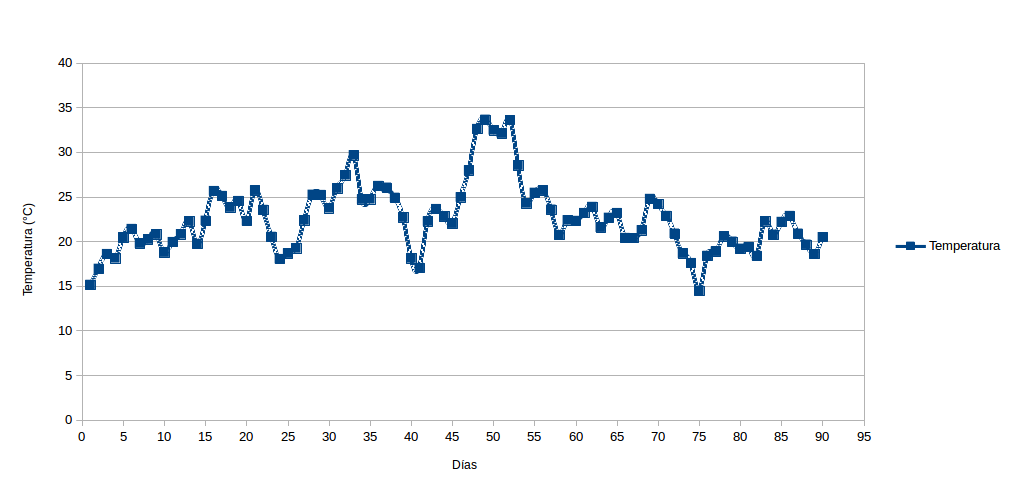
\includegraphics[width=\textwidth]{capitulo-6/graphics/temperatura-variable-90.png}
    \caption{\label{fig:var-temperatura}Variación de la temperatura durante un periodo de 90 días.}
\end{figure}

En general se pudo observar una duración de 4,07 días para su fase de huevo, 10,13 días para la
fase larval y 2,74 días para fase pupal. La duración del ciclo gonotrófico correspondiente a
hembras nulíperas y paridas fue de 4,75 y 3,43 días respectivamente.

En la \figref{fig:temp-var-poblacion} se puede observar el comportamiento creciente y decreciente
de la población de mosquitos en relación al tiempo. El decrecimiento de la población de individuos
en etapas inmaduras se encuentra influenciado por la mortalidad diaria y emergencia a adultos,
donde esta última causa el crecimiento de la población de adultos. La oviposición de las hembras
adultas, pertenecientes a la población de adultos, es la causante del crecimiento de la población
de individuos en etapas inmaduras. El decrecimiento de la población de adultos es causada por la
mortalidad diaria.

\begin{figure}[!htbp]
    \centering
    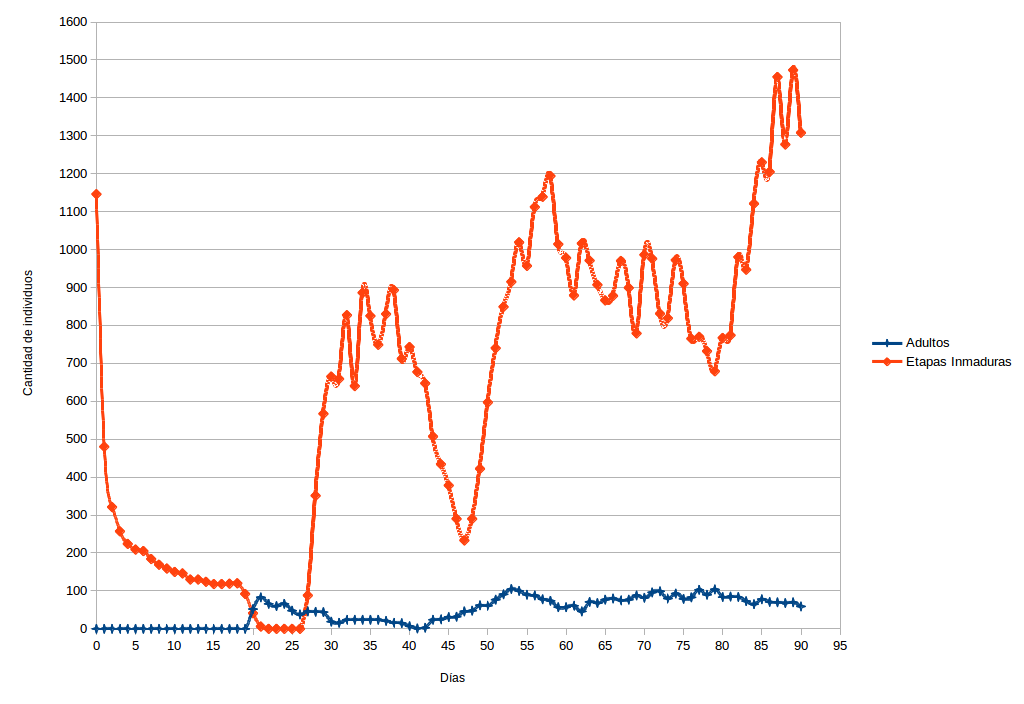
\includegraphics[width=\textwidth]{capitulo-6/graphics/temp-var-90-poblacion.png}
    \caption{\label{fig:temp-var-poblacion} Análisis del comportamiento de la población de mosquitos durante un periodo de 90 días a temperaturas variables.}
\end{figure}

En la \figref{fig:temp-var-generacion} se puede observar comportamiento correspondiente de las
generaciones de mosquitos pertenecientes a la población. En general se pudieron observar 4
generaciones de individuos en etapas inmaduras y 3 generaciones de adultos. La primera generación
corresponde a los individuos pertenecientes a la población inicial, la segunda generación
corresponde a los descendientes la primera generación, producto de la oviposición de las hembras
adultas emergentes de la población inicial. La tercera generación corresponde a los descendientes
de la segunda generación. La cuarta y última generación se encuentra compuesta únicamente por
individuos en etapas inmaduras, ya que ninguno de sus individuos emergió para convertirse en adulto.

\begin{figure}[!htbp]
    \centering
    \begin{subfigure}[b]{\textwidth}
        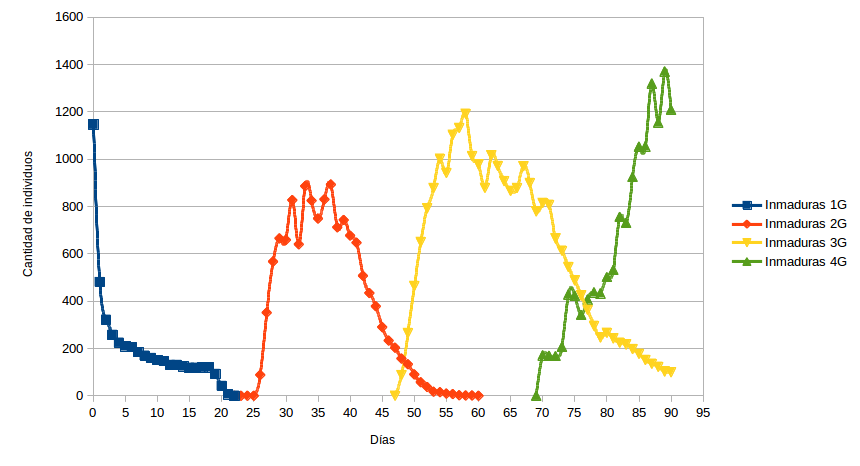
\includegraphics[width=\textwidth]{capitulo-6/graphics/temp-var-90-generacion-inmaduras.png}
        \caption{\label{fig:temp-var-inmaduras-generacion}Crecimiento generacional de la población de individuos en etapas inmaduras a temperatura variable.}
    \end{subfigure}
    ~~~~
    \begin{subfigure}[b]{\textwidth}
        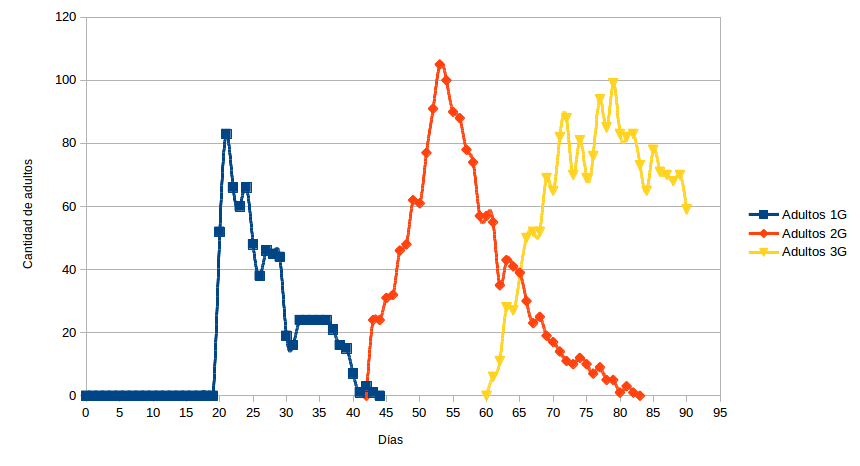
\includegraphics[width=\textwidth]{capitulo-6/graphics/temp-var-90-generacion-adultos.png}
        \caption{\label{fig:temp-var-adultos-generacion}Crecimiento generacional de la población de adultos a temperatura variable.}
    \end{subfigure}

    \caption{\label{fig:temp-var-generacion} Análisis generacional de la población de mosquitos durante un periodo de 90 días a temperatura variable.}
\end{figure}
